\documentclass[12pt,a4paper]{scrartcl}
\usepackage[utf8]{inputenc}
\usepackage[english,russian]{babel}
\usepackage{indentfirst}
\usepackage{misccorr}
\usepackage{graphicx}
\usepackage{amsmath}
\usepackage{multirow}
\usepackage{pgfplots}
\usepackage{parskip}
\usepackage[top=1cm, bottom=1cm, left=1cm, right=1cm]{geometry}
\pgfplotsset{compat=1.9}

\begin{document}
	\graphicspath{{pic/}, {~/Pictures/TeXImgs/}}
	
	\newcommand{\ms}{\mathstrut}
	\newcommand{\msp}{\hspace{0.5cm}}
	\newcommand{\al}{\alpha}
	\newcommand{\dg}{^\circ}
	\newcommand{\dif}{\mathrm{d}}
	\newcommand{\qd}[2]{^{\frac{#1}{#2}}}
	\newcommand{\qdm}[2]{^{-\frac{#1}{#2}}}
	\newcommand{\lm}[2]{\underset{#1 \rightarrow #2}{\lim}}
	\newcommand{\sfrac}[2]{\dfrac{\strut #1}{\strut #2}}
	\newcommand{\equal}[1]{\overset{(#1)}{=}}
	\newcommand{\linevdots}{\ \raisebox{-.08\height}{\vdots}\ }
	\newcommand{\linecvdots}{\ \raisebox{-.08\height}{\vdots}\hspace{-0.13cm}\raisebox{.15\height}{\cancel{\phantom{a}}\hspace{0.06cm}}}
	\newcommand{\combox}[1]{\ms \msp \msp \begin{minipage}{0.95\linewidth}
			#1
	\end{minipage}}
	
	\newtheorem{pr}{Задача}
	\newtheorem{ex}{Пример}
	\newtheorem{dfn}{Def}
	\newtheorem{theorem}{Th}
	
	\newenvironment{slv}{\ms \msp \textit{Решение:}}{}
	\newenvironment{proof}{\ms \msp \textit{Доказательство: }}{\hfill $\square$}
	
	\begin{titlepage}
		
		\vspace*{\fill}
		
		\begin{center}
			
\includegraphics[scale=0.8]{MIPT.png}
			\\[0.7cm]\Huge Московский Физико-Технический Институт\\(национальный исследовательский университет)
			\\[2cm]\LARGE Отчет по эксперименту
			\\[0.5cm]\noindent\rule{\textwidth}{1pt}
			\\\Huge\textbf{Закон Кюри–Вейсса}
			\\[-0.5cm]\noindent\rule{\textwidth}{1pt}
		\end{center}
		
		\begin{flushleft}
			\textit{Работа №3.4.2; дата: 16.09.22}\hfill\textit{Семестр: 3}
		\end{flushleft}
		
		\vspace*{\fill}
		
		\begin{flushleft}
			Выполнил: \hspace{\fill} Группа:
			\\Кошелев Александр \hspace{\fill} Б05-105
		\end{flushleft}
	\end{titlepage}
	
	%Страница 2
	
	\begin{flushleft}
		\footnotesize{Закон Кюри–Вейсса} \hspace{\fill} \footnotesize{2}
		\\[-0.3cm]\noindent\rule{\textwidth}{0.3pt}
	\end{flushleft}
	
	\section{Аннотация}
	
	\textbf{Цель работы: }
	
	Изучение температурной зависимости магнитной восприимчивости ферромагнетика выше точки Кюри.
	
	\textbf{Схема установки:}
	\begin{center}
		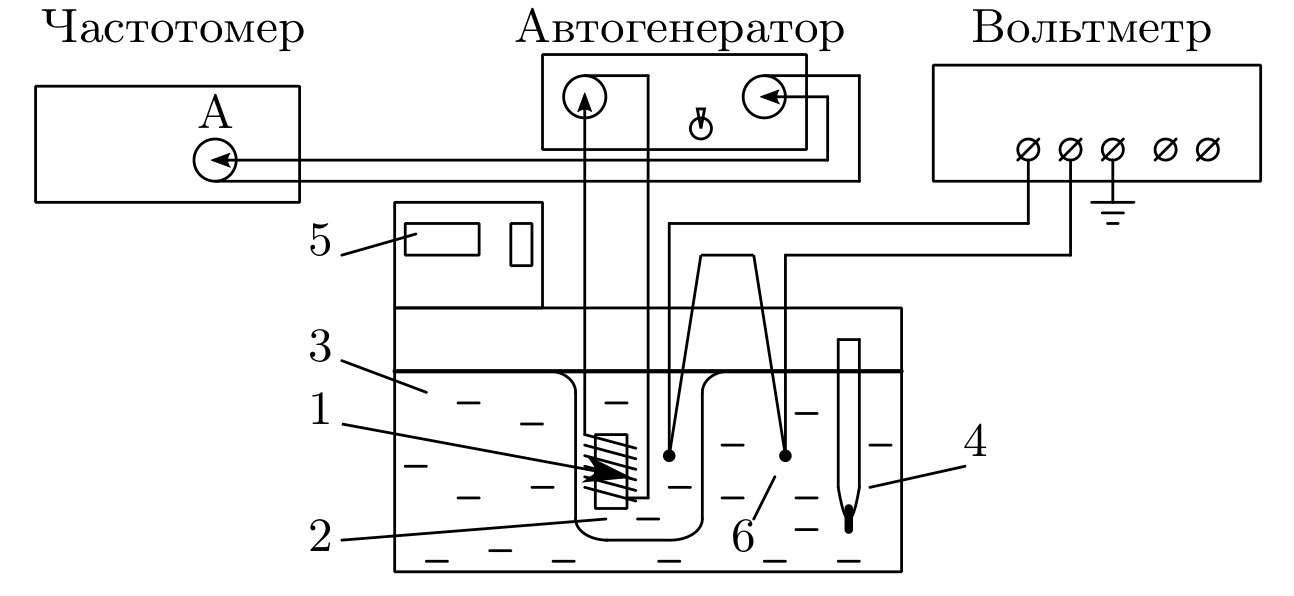
\includegraphics[scale=0.32]{PIC_1.png}
		\\\textbf{Рис. 1:} Схема установки
	\end{center}	
		
	Исследуемый ферромагнитный образец (гадолиний) расположен внутри пустотелой катушки самоиндукции, которая служит индуктивностью колебательного контура, входящего в состав $LC$-автогенератора.
	
	Гадолиний является хорошим проводником электрического тока, а рабочая частота генератора достаточно велика (50 кГц), поэтому для уменьшения вихревых токов образец из готовлен
	из мелких кусочков размером 0.5 мм. Катушка 1 с образцом помещена в стеклянный сосуд 2,
	залитый трансформаторным маслом. Масло предохраняет образец от окисления и способствует ухудшению электрического контакта между отдельными частичками образца. Кроме того,
	оно улучшает тепловой контакт между образцом и термостатируемой (рабочей) жидкостью 3 в
	термостате. Ртутный термометр 4 используется для приближенной оценки температуры. При
	изменении температуры меняется магнитная восприимчивость образца $\chi$, а следовательно, самоиндукция катушки и период колебаний $\tau$ автогенератора. Для измерения периода используется частотомер.
	
	Для нагрева используется термостат. Температура исследуемого образца всегда несколько
	отличается от температуры дистиллированной воды в сосуде. После того как вода достигла
	заданной температуры, идёт медленный процесс выравнивания температур образца и воды.
	Разность их температур контролируется с помощью медноконстантановой термопары 6 и цифрового вольтметра. Один из спаев термопары находится в тепловом контакте с образцом , а другой погружён в воду. Концы термопары подключены к цифровому вольтметру. Рекомендуется измерять период колебаний автогенератора в тот момент, когда указанная разность
	температур становится $\leqslant$ 0.5$\, ^\circ \mathrm{C}$. Чувствительность термопары $k$ = 24 К/мВ.
		
	\textbf{В работе используются:}
	
	Катушка самоиндукции с образцом из гадолиния, термостат, частометр, цифровой вольтметр, $LC$-автогенератор, термопара медь-константин.
	
	\newpage
	
	%Страница 3
	
	\begin{flushleft}
		\footnotesize{Закон Кюри–Вейсса} \hspace{\fill} \footnotesize{3}
		\\[-0.3cm]\noindent\rule{\textwidth}{0.3pt}
	\end{flushleft}
	
	\section{Теоретические сведения}
	
	Ферромагнетики обладают свойством намагничиваться даже в слабых магнитных полях.
	Впервые количественную теорию ферромагнетизма разработал французский физик Вейсс в
	1907 году. В настоящей работе для изучения температурной зависимости магнитной восприимчивости ферромагнетика выше точки Кюри (то есть в парамагнитной области) используется
	закон Кюри-Вейсса (который назван так по аналогии с законом Кюри для парамагнетиков).
	
	\begin{equation}
		\chi = \sfrac{C}{T - \Theta_p} \sim \sfrac{1}{T - \Theta_p}
	\end{equation}
	
	где $\chi$ -- магнитная восприимчивость, $C$ -- постоянная Кюри, зависящая от вещества, $T$ --
	абсолютная температура в кельвинах, $\Theta_p$ — парамагнитная температура Кюри в кельвинах.
	
	При повышении температуры $T$ возрастает дезориентирующее действие теплового движения частиц, и магнитная восприимчивость парамагнетиков убывает, в простейшем случае (в постоянном магнитном поле) пo закону Кюри.
	
	При $T \rightarrow 0$ тепловое движение всё меньше препятствует магнитным моментам атомов ориентироваться
	в одном направлении при сколь угодно слабом внешнем поле. 
	
	\begin{center}
		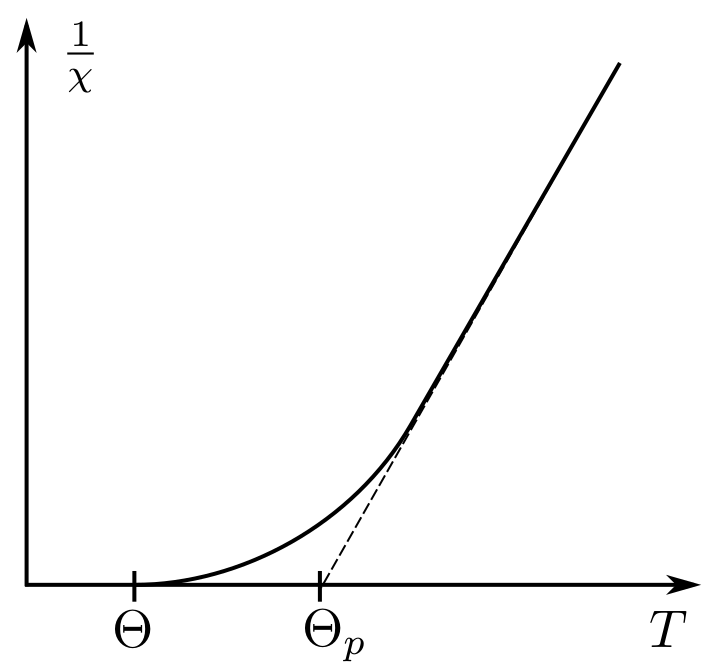
\includegraphics[scale=0.2]{PIC_2.png}
		\\\textbf{Рис. 2:} График реальной зависимости $\frac{1}{\chi}(T)$
	\end{center}
	
	В ферромагнетиках (под влиянием обменных
	сил) это происходит при понижении температуры не до	абсолютного нуля, а до температуры Кюри $\Theta$, в котором добавка к температуре $\Theta_p$ — некая температура, называемая парамагнитной точкой Кюри. Она близка к $\Theta$, но немного больше ее. Оказывается, что у ферромагнетиков закон Кюри должен быть заменён	законом Кюри-Вейсcа (1). Эта формула хорошо описывает поведение ферромагнитных веществ после их перехода в парамагнитную фазу при заметном удалении	температуры от 0, но недостаточно точна при $T \approx \Theta$.
	
	В нашей работе изучается температурная зависимость $\chi(T)$ гадолиния при температурах выше точки Кюри. Выбор материала определяется тем, что его точка Кюри лежит в интервале комнатных температур.
	
	
	Свяжем теперь периоды колебаний автогенератора с магнитной восприимчивостью. Связь самоиндукций катушки с магнитной восприимчивостью такова:
	
	$$L - L_0 \propto \mu - 1 = \chi$$
	
	А значит, с учетом формулы периода $\tau = 2\pi \sqrt{LC}$, получаем следующее соотношение:
	
	$$\chi \propto \tau^2 - \tau_0 ^2$$
	
	\newpage
	
	%Страница 4
	
	\begin{flushleft}
		\footnotesize{Закон Кюри–Вейсса} \hspace{\fill} \footnotesize{4}
		\\[-0.3cm]\noindent\rule{\textwidth}{0.3pt}
	\end{flushleft}
	
	\section{Проведение эксперимента}
	
	\paragraph{Начальные данные} \hfill
	
	Обозначим начальные данные нашей установки, для удобства, в виде таблицы.
	
	\begin{center}
		\begin{tabular}{|c|c|c|c|c|}
			\hline
			$k$, К/мВ & $\tau_0$, мкс & $\sigma_U$, мВ & $\sigma_{T_{\text{терм}}}$, К & $\sigma_\tau$, мкс
			\\\hline
			24 & 6.95636 & 0.012 & 0.01 & 0.01
			\\\hline
		\end{tabular}
		\\\textbf{Табл. 1:} Начальные данные установки
	\end{center}

	Необходимо, чтобы разница температур между образцом и термостатом была не более половины градуса, то вычисляем максимальное напряжение термопары, при котором допустимо измерение:
	
	$$U_{\mathrm{max}} = \sfrac{(\Delta T)_{\mathrm{max}}}{k} \approx 0.021\, \text{мВ}$$
	
	Теперь снимем показания вольтметра и частометра при разных температурах термостата, повышая после каждого измерения температуру термостата на два градуса. При этом температуру образца будем считать по
	следующей формуле:
	
	$$T = T_{\text{терм}} + kU$$
	
	Причем погрешности считаются как:
	
	$$\sigma_T = \sqrt{\sigma_{\text{терм}}^2 + (k\sigma_U)^2}$$
	
	$$\sigma_{\frac{1}{\tau^2 - \tau_0^2}} = \sfrac{2\tau}{(\tau^2 - \tau_0^2)} \sigma_{\tau}$$
	
	Результаты оформим в таблицу:
	
	\begin{center}
		\begin{tabular}{|c|c|c|c|c|c|}
			\hline
			$i$ & $T_{\text{терм}}$, $^\circ\mathrm{C}$ & $U$, мВ & $\tau$, мкс & $T$, $^\circ\mathrm{C}$ & $\frac{1}{\tau^2 - \tau_0^2}$, мкс$^{-2}$
			\\\hline
			1 & 14.76 $\pm$ 0.01 & -0.003 $\pm$ 0.001 & 7.960 $\pm$ 0.010 & 14.69 $\pm$ 0.03 & 0.064 $\pm$ 0.001
			\\\hline
			2 & 16.10 $\pm$ 0.01 & -0.003 $\pm$ 0.001 & 7.910 $\pm$ 0.010 & 16.03 $\pm$ 0.03 & 0.067 $\pm$ 0.001
			\\\hline
			3 & 18.11 $\pm$ 0.01 & -0.009 $\pm$ 0.001 & 7.790 $\pm$ 0.010 & 18.04 $\pm$ 0.03 & 0.077 $\pm$ 0.001
			\\\hline
			4 & 20.17 $\pm$ 0.01 & -0.010 $\pm$ 0.001 & 7.610 $\pm$ 0.010 & 20.10 $\pm$ 0.03 & 0.098 $\pm$ 0.002
			\\\hline
			5 & 22.09 $\pm$ 0.01 & -0.013 $\pm$ 0.001 & 7.410 $\pm$ 0.010 & 22.02 $\pm$ 0.03 & 0.140 $\pm$ 0.003
			\\\hline
			6 & 24.07 $\pm$ 0.01 & -0.013 $\pm$ 0.001 & 7.240 $\pm$ 0.010 & 24.00 $\pm$ 0.03 & 0.214 $\pm$ 0.007
			\\\hline
			7 & 26.09 $\pm$ 0.01 & -0.013 $\pm$ 0.001 & 7.160 $\pm$ 0.010 & 26.02 $\pm$ 0.03 & 0.284 $\pm$ 0.012
			\\\hline
			8 & 28.09 $\pm$ 0.01 & -0.006 $\pm$ 0.001 & 7.130 $\pm$ 0.010 & 28.02 $\pm$ 0.03 & 0.330 $\pm$ 0.016
			\\\hline
			9 & 30.07 $\pm$ 0.01 & -0.013 $\pm$ 0.001 & 7.090 $\pm$ 0.010 & 30.00 $\pm$ 0.03 & 0.397 $\pm$ 0.022
			\\\hline
			10 & 35.07 $\pm$ 0.01 & -0.012 $\pm$ 0.001 & 7.013  $\pm$ 0.010 & 35.00 $\pm$ 0.03 & 0.598 $\pm$ 0.050
			\\\hline
			11 & 40.07 $\pm$ 0.01 & -0.015 $\pm$ 0.001 & 6.999  $\pm$ 0.010 & 40.00 $\pm$ 0.03 & 0.799 $\pm$ 0.089
			\\\hline
		\end{tabular}
		\\\textbf{Табл. 2:} Проведение эксперимента
	\end{center}
	
	\newpage
	
	%Страница 5
	
	\begin{flushleft}
		\footnotesize{Закон Кюри–Вейсса} \hspace{\fill} \footnotesize{5}
		\\[-0.3cm]\noindent\rule{\textwidth}{0.3pt}
	\end{flushleft}
	
	По полученным данным построим график зависимости $\frac{1}{\tau^2 - \tau_0^2}(T)$:
	
	\begin{center}
		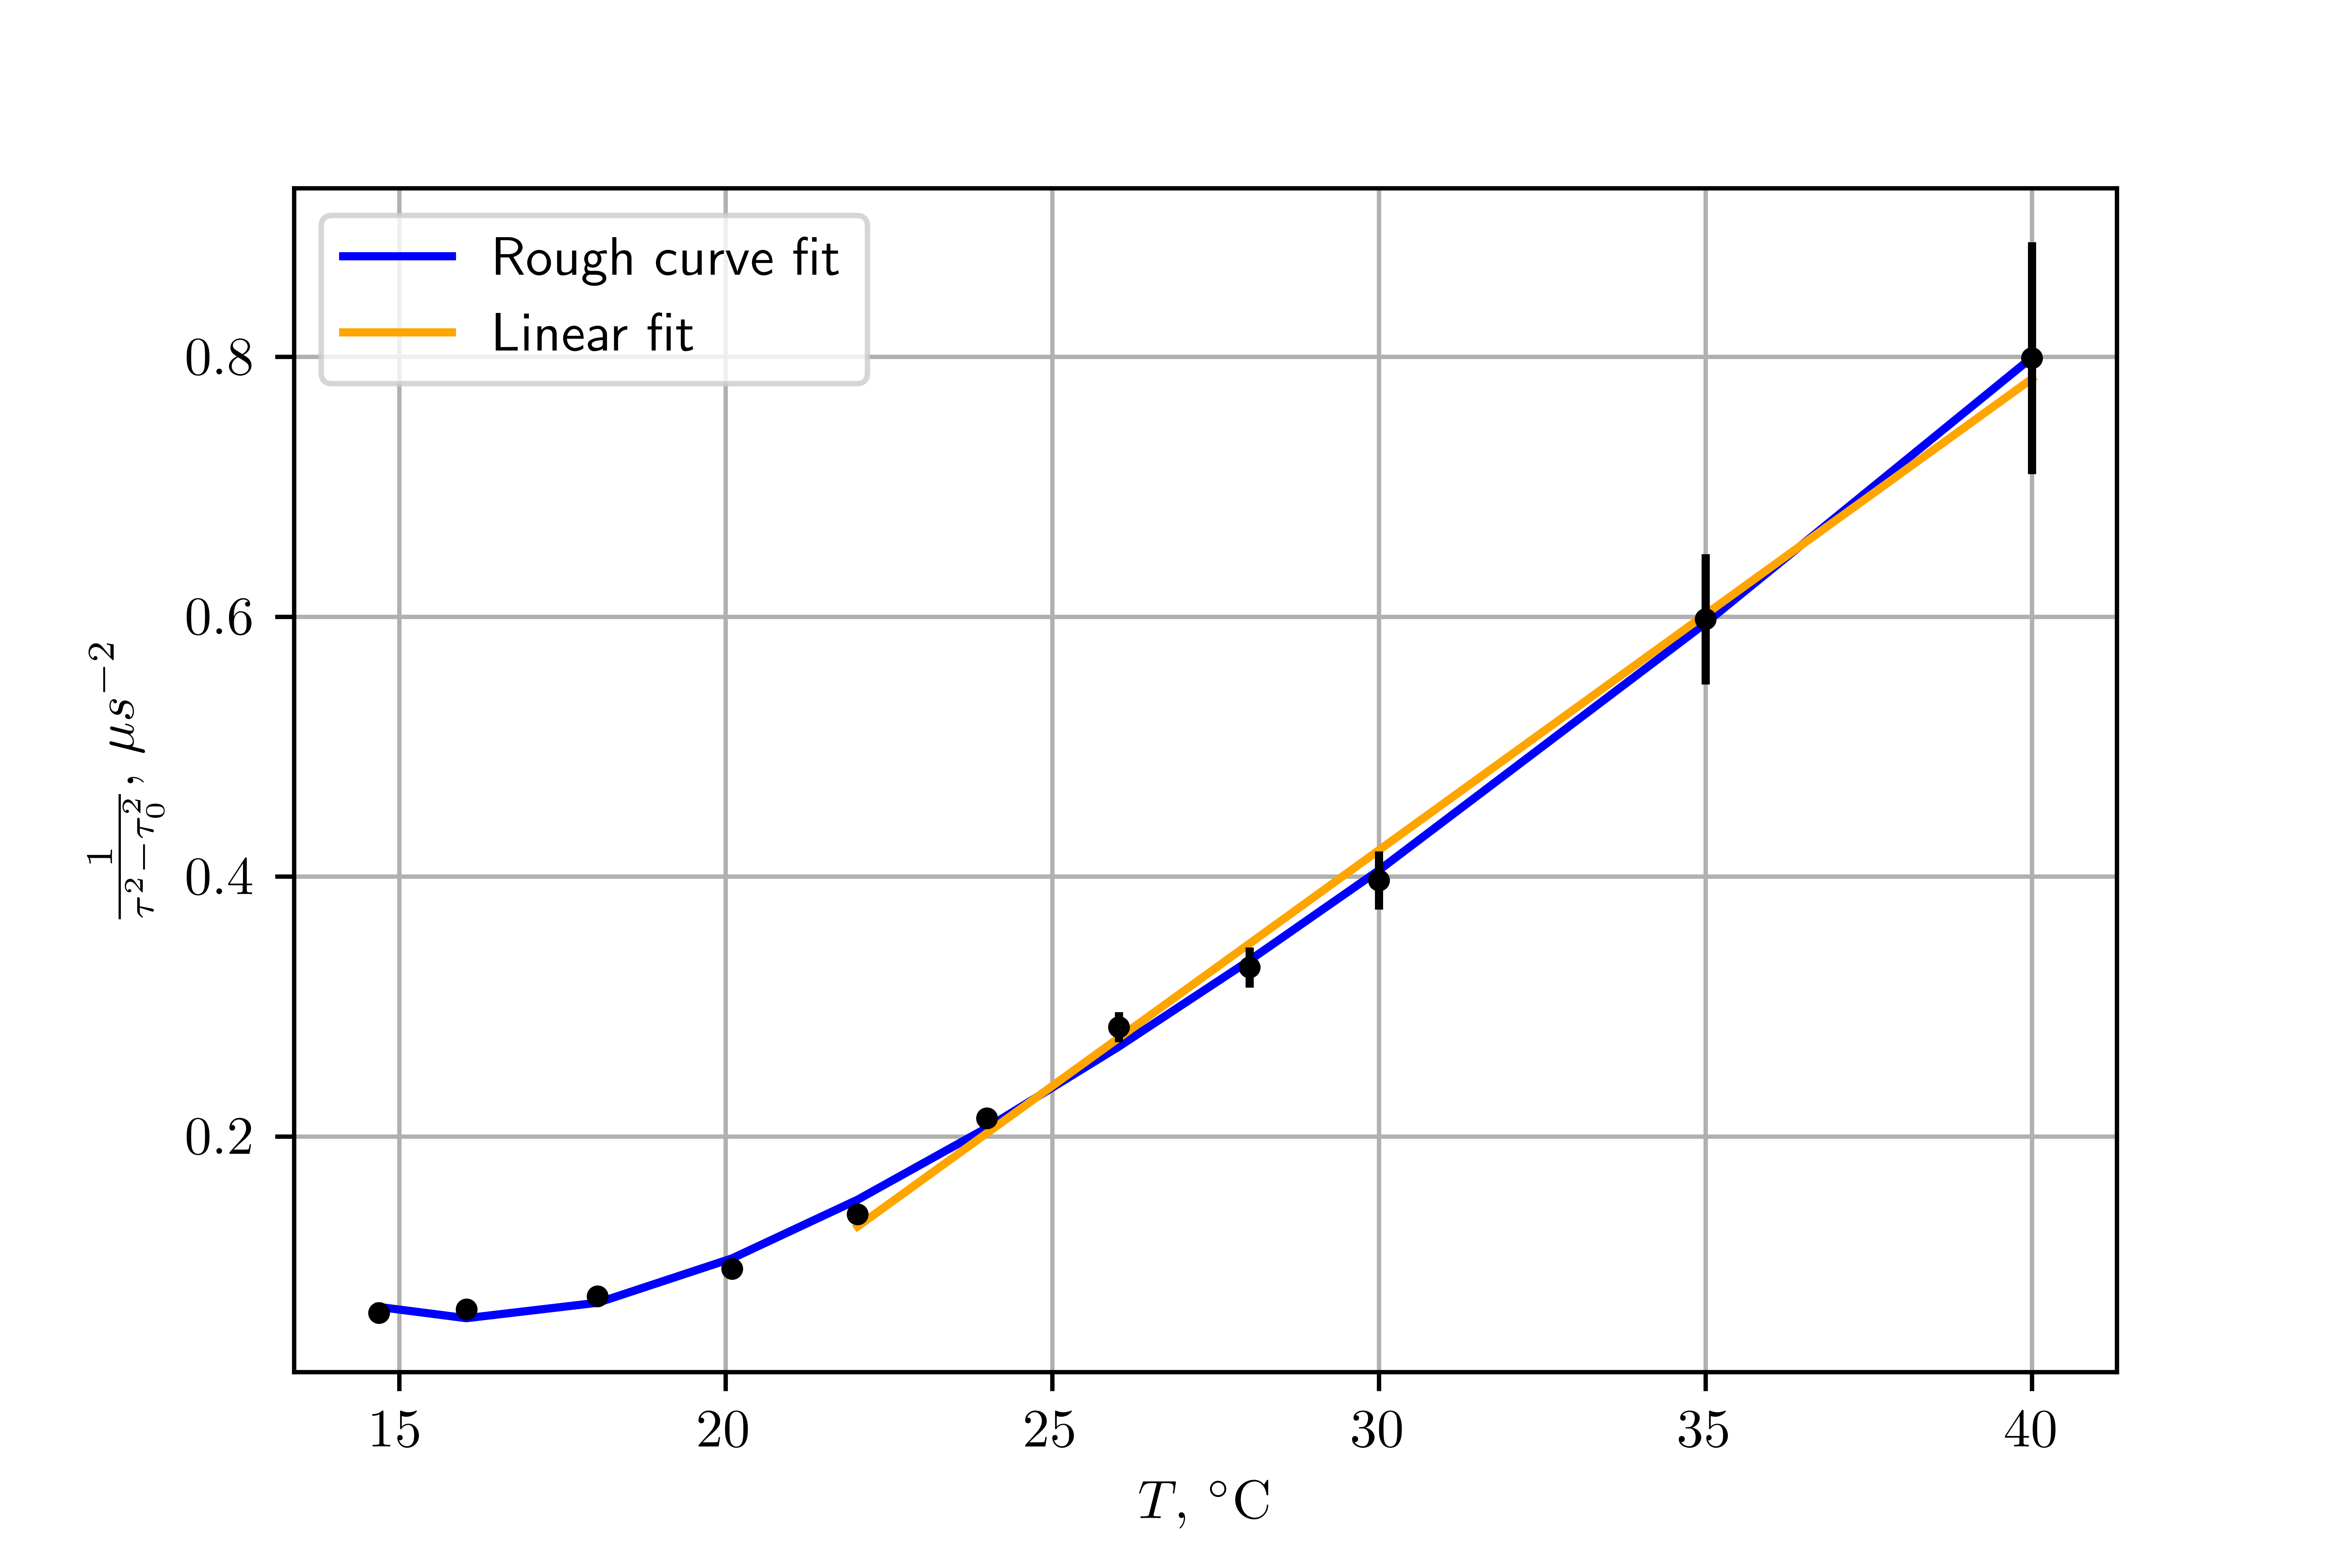
\includegraphics[scale=1]{PIC_3.png}
		\\\textbf{Рис. 3:} График зависимости $\frac{1}{\tau^2 - \tau_0^2}(T)$
	\end{center}
	
	При этом проведем линейную аппроксимацию  части графика, близкой к линейной. Прямая задается уравнением $y = kx + b$, ее параметры:
	
	\begin{center}
		\begin{tabular}{|c|c|}
			\hline
			$k$, $\mu s^{-2} K^{-1}$ & $b$, $\mu s^{-2}$
			\\\hline
			0.0363 $\pm$ 0.0011 & -0.6685 $\pm$ 0.0326
			\\\hline
		\end{tabular}
		\\\textbf{Табл. 3:} Линейная аппроксимация
	\end{center}

	Таким образом, параегнитная температура Кюри:
	
	$$\Theta_p = \sfrac{-b}{k} = (18.48 \pm 0.95) ^\circ \mathrm{C} = (291.48 \pm 0.95) \mathrm{K}$$
	
	При этом погрешность конечного результата:
	
	$$\sigma_{\Theta_p} = \sqrt{\left(\sfrac{\sigma_b}{k}\right)^2 + \left(\sfrac{b\sigma_k}{k^2}\right)^2}$$
	
	\section{Выводы}
	
	В ходе работы была исследована зависимость $\frac{1}{\tau^2 - \tau_0^2}(T)$, был построен график этой зависимости. Путем аппроксимации линейной части зависимости получена парамагнитная точка Кюри для гадолиния:
	
	$$\Theta_p = (18.48 \pm 0.95) ^\circ \mathrm{C} = (291.48 \pm 0.95) \mathrm{K}$$
	
	Результат хорошо согласуется с табличным значением точки Кюри $\Theta = 19 ^\circ \mathrm{C}$.
	
\end{document}